\documentclass[12pt, a4paper]{article}
\usepackage[utf8]{inputenc}
\usepackage{graphicx}
\usepackage{amsmath}
\graphicspath{ {img/} }

\title{First document}
\author{PIN-CHUN, HSU}
\date{April 2017}
\begin{document}

\maketitle

First document. This is a simple example, with no
extra parameters or packages included. %comment here
try

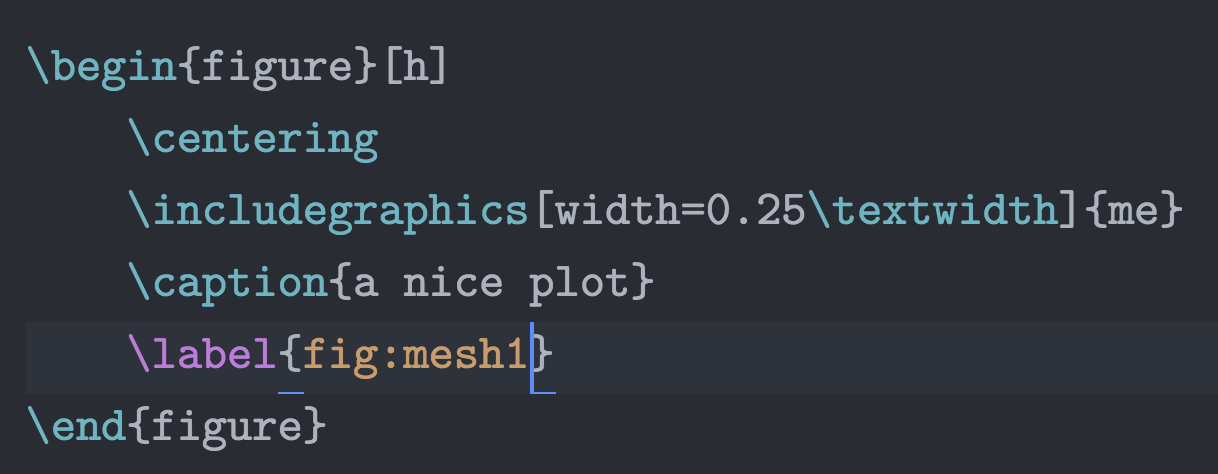
\includegraphics[width=50mm,scale=0.5]{tmp}

test
Some of \textbf{Bold texts}
and some \underline{Underline texts}
and more \textbf{\textit{Text it}}
\textbf{ already in bold font but still can \emph{Emphasize} something}

\begin{figure}[h]
    \centering
    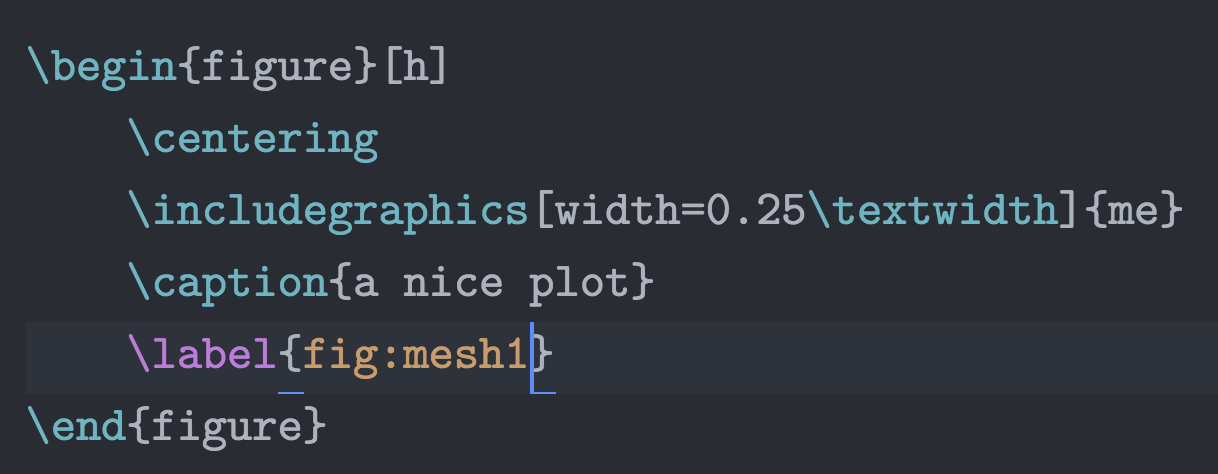
\includegraphics[width=0.25\textwidth]{tmp}
    \caption{a nice plot}
    \label{fig:mesh1}
\end{figure}

As you can see in the figure \ref{fig:mesh1}, the
function grows near 0. Also, in the page \pageref{fig:mesh1}
is the same example.

\begin{itemize}
  \item The individual entries are indicated with a black dot, a so-called bullet.
  \item The text in the entries may be of any length.
\end{itemize}

\begin{enumerate}
  \item This is the first entry in our list
  \item The list numbers increase with each entry we add
\end{enumerate}

In physics, the mass-energy equivalence is stated
by the equation $E=mc^2$, discovered in 1905 by Albert Einstein.
math like $\frac{2 \pi R}{\mu_0 i}$

The mass-energy equivalence is described by the famous equation

$$E=mc^2$$
discovered in 1905 by Albert Einstein.
In natural units ($c = 1124$), the formula expresses the identity

\begin{equation}
E=m
\end{equation}

Subscripts in math mode are written as $a_b$ and superscripts are written as $a^b$. These can be combined an nested to write expressions such as

$$T_{j_1 j_2 \dots j_q}^{i_1 i_2 \dots i_p} =
T(x^{i_1}, \dots, x^{i_p}, e_{j_1}, \dots, e_{j_q})$$

We write integrals using $\int$ and fractions using $\frac{a}{b}$. Limits are placed on integrals using superscripts and subscripts:

$$\int_0^1 \frac{1}{e^x} = \frac{e-1}{e}$$

Lower case Greek letters are written as $\omega$ $\delta$ etc. while upper case Greek letters are written as $\Omega$ $\Delta$.

Mathematical operators are prefixed with a backslash as $\sin(\beta)$, $\cos(\alpha)$, $\log(x)$ etc.

\begin{center}
\begin{tabular}{ c c c }
 cell1 & cell2 & cell3 \\
 cell4 & cell5 & cell6 \\
 cell7 & cell8 & cell9
\end{tabular}
\end{center}
Mathematical operators are prefixed with a backslash as $\sin(\beta)$, $\cos(\alpha)$, $\log(x)$ etc.
\begin{center}
\begin{tabular}{ |c|c|c| }
 cell1 & cell2 & cell3 \\
 \hline
 cell4 & cell5 & cell6 \\
 \hline
 cell7 & cell8 & cell9
\end{tabular}
\end{center}

Table \ref{table:data} is an example of referenced \LaTeX{} elements.

\begin{table}[h!]
\centering
\begin{tabular}{||c c c c||}
 \hline
 Col1 & Col2 & Col2 & Col3 \\ [0.5ex]
 \hline\hline
 1 & 6 & 87837 & 787 \\
 2 & 7 & 78 & 5415 \\
 3 & 545 & 778 & 7507 \\
 4 & 545 & 18744 & 7560 \\
 5 & 88 & 788 & 6344 \\ [1ex]
 \hline
\end{tabular}
\caption{Table to test captions and labels}
\label{table:data}
\end{table}

\section{Introduction}

This is the first section.

Lorem  ipsum  dolor  sit  amet,  consectetuer  adipiscing
elit.   Etiam  lobortisfacilisis sem.  Nullam nec mi et
neque pharetra sollicitudin.  Praesent imperdietmi nec ante.
Donec ullamcorper, felis non sodales...
\section{Second Section}

Lorem ipsum dolor sit amet, consectetuer adipiscing elit.
Etiam lobortis facilisissem.  Nullam nec mi et neque pharetra
sollicitudin.  Praesent imperdiet mi necante...

\subsection{First Subsection}
Praesent imperdietmi nec ante. Donec ullamcorper, felis non sodales...

\section*{Unnumbered Section}
Lorem ipsum dolor sit amet, consectetuer adipiscing elit.
Etiam lobortis facilisissem

\end{document}
